\documentclass[finalversion]{usetex-v1}
%\usepackage[top=1in, bottom=1in, left=1.25in, right=1.25in]{geometry}
\usepackage[colorlinks,linkcolor=red,anchorcolor=blue,citecolor=green,urlcolor=black]{hyperref}
\usepackage{epsfig}
\usepackage{breakurl}
%% Define a new 'leo' style for the package that will use a smaller font.
\makeatletter
\def\url@leostyle{%
  \@ifundefined{selectfont}{\def\UrlFont{\sf}}{\def\UrlFont{\small\ttfamily}}}
\makeatother
%% Now actually use the newly defined style.
\urlstyle{leo}
%\linespread{1.2}
%\setlength{\parskip}{1ex}
\begin{document}
\title{foo}
\author{bar}
\date{}
\maketitle

\begin{abstract}
Virtualization has became the engine behind many cloud computing platforms.
In a virtualized computing environment, virtual machines
operate on virtual disks, so backing up user data is done by constantly 
taking snapshots of those virtual disks. Because such VM snapshots are huge in
terms of both quantity and individual sizes, snapshot storage would cost tremendous amount 
of space without deduplication.
Current snapshot deduplication is mainly done through copy-on-write 
on fixed-size disk blocks. Such solutions are fast but unable to handle the
 cross VM and inner-block data duplications. In addition, storing VM images and their snapshots
in the same storage engine reduce the underline design flexibility since these two kinds of data
have distinct access requirements.

In this paper, we first perform a large scale study in production VM clusters 
to show that cross VM data duplication is severe due to they have large amount of
common data. Then our data analysis finds out that the overall data duplication pattern follows the Zipf's law.
Base on these discoveries, we propose a snapshot storage deduplication scheme using variable-size chunking
to address the above problem efficiently.
We eliminate the majority of cross VM data duplication by pre-select
a small set of frequently seen chunks to dedup against, and we also remove
many inner-block duplication using smaller chunking granuarity and locality.
Experiment shows our design can achieve high deduplication ratio and throughput
without incuring significant overhead to the runtime VM environment.
\end{abstract}

\section{Introduction}
In a cluster-based cloud environment such as ones provided by Amazon EC2\cite{AmazonEC2} 
and Alibaba Aliyun\cite{Aliyun},
each physical machine runs a number  of virtual machines as  instances of a guest operating system 
and their  virtual hard disks are represented as virtual disk image files in the host operating system.
%virtual disk image files (e.g. .vhd, .vmdk) in the host operating system.
%Backup  of virtual disks is relatively straightforward since
%these image files are stored as regular files from the external point of view,
%backing up VM's data is mainly done by taking snapshots of virtual disk images.

%A snapshot preserves the data of a VM's file system at a specific point in time. 
%VM snapshots can be  backed up  incrementally by comparing blocks from one version to another 
%and only the blocks that have changed from the previous version of snapshot will be saved~\cite{Clements2009,Vrable2009}. 
Frequent  snapshot backup of virtual disk images  can increase  the service reliability. 
For example, the Aliyun cloud , which is  the largest cloud service provider by Alibaba in China, 
automatically conducts  the backup of virtual disk images to all active users every day.
The cost of supporting a large number of concurrent backup streams is high
because of the huge storage demand and  
Using a separate  backup service with full deduplication support~\cite{venti02,bottleneck08}
can effectively identify content duplicates among snapshots and  remove 
redundant storage content,  but the solution can be expensive and there is a large amount of 
network traffic to transfer  data from the host machines to the backup facility
before duplicates are removed.


This paper seeks for a low-cost architecture option and considers that
a backup service collocates  on  the cloud cluster with a minimum resource usage. 
%Since most of backup data is not used in practice, system resource in such a service is not fully utilized.
The dirty bit approach~\cite{??}  which checks the version difference can effectively remove
duplicates while using content fingerprints can significantly compress more~\cite{Bottlneck08}.
On the other hand, comparing fingerprints  adds significant  memory cost. 
Since each physical machine in a cluster  hosts many VMs, memory contention happens frequently.
Cloud providers often wish that the backup service only consumes  small or modest resources
with a minimal impact to the existing cloud services.  A 
recent study using subsampling~\cite{Guo2011}  can significantly reduce the memory requirement.
Another issue is that after deduplication, the most of data blocks are shared by many virtual machines.
Failure of such blocks would  have a catastrophic effect and many snapshots of virtual machines would be affected.
Furthermore, 
%that deletion of old snapshots compete for computing resource as well. That is because data dependence created
deletion of old snapshots compete for computing resource as well and that  needs
to be considered. That is  because data dependence created
by duplicate relationship among snapshots  adds processing complexity.
% especially when  VMs can migrate around in the cloud.

The paper proposes an integrated approach which uses  multiple duplicate detection strategies
integrating  version  detection, small-scope inner VM duplicate comparison
and controlled cross-VM comparison. 
The key idea of this approach is to localize duplicate detection within each virtual machine as much as possible
and minimize memory usage while delivering a decent deduplication efficiency. 
That brings the benefits for parallelism  utilization and fault isolation.
Our deletion strategy uses a double Boomer filer strategy for periodic mark-and-sweeping of expired data blocks.
We have developed a prototype system that runs a cluster of Linux machines running Zen.
The backup storage uses a standard distributed file system  with data replication and
we allocate more  replicas for the commonly-shared  data blocks among VM snapshots to enhance fault tolerance.



%************** Paper sections summary
%THIS NEEDS MODIFICATION
The rest of this paper is organized as follows.
Section~\ref{review} reviews background and related work.
Section~\ref{sec:framework}  discusses the  design framework and system architecture.
Section~\ref{sec:model}  analyzes the benefit of our approach for fault isolation. 
Section~\ref{exper} is our experimental evaluation that compare with the other approach.
Section~\ref{conc}  concludes this paper.

%We are seeking Unlike the previous work dealing with general file-level backup and deduplication, our problem is focused on 
%virtual disk image backup. Although we treat each virtual disk  as a file logically, its size is very large.
%On the other hand, we need to support parallel backup of a large number of virtual disks in a cloud every day. 
%One key requirement we face at Alibaba Aliyun is that VM snapshot backup should only use a minimal amount of system
%resources so that most of resources is kept for regular cloud system services or applications.
%Thus our objective is to exploit the characteristics of VM snapshot data and
%pursue a cost-effective deduplication solution. 
%Another goal  is to decentralize VM snapshot backup and  localize  deduplication as much as possible,

%,extreme_binning09,sparseindex09
\comments{
By observations on the VM snapshot data from production cloud, we found snapshot data duplication 
can be easily classified into two categories: \emph{inner-VM} and \emph{cross-VM}. Inner-VM duplication
exists between VM's snapshots, because the majority of data are unchanged during each backup period. 
On the other hand, Cross-VM duplication is mainly due to widely-used software and libraries such as Linux and MySQL.
As the result, different VMs tend to backup large amount of highly similar data.

With these in mind, we  have developed a distributed multi-level solution to conduct 
segment-level  and block-level inner-VM  deduplication to localize the deduplication effort when possible.
It then makes cross-VM deduplication by excluding a small number of
popular common data blocks from being backed up. Our study shows that common data blocks
occupy significant amount of storage space while they only take
a small amount of resources to deduplicate.
Separating deduplication into multi levels effectively accomplish the major space saving goal
compare the global complete deduplication scheme, at the same time it makes
the backup of different VMs to be independent for better fault tolerance.

The following table shows the strength and weakness of some well-know deduplication systems:
\begin{table}
    \begin{tabular}{|l|l|l|l|}
        \hline
        ~           & Scalability & Low-cost & Full Dedup \\ \hline
        DDFS        & N           & N        & Y          \\ 
        Ex-bin      & Y           & Y        & N          \\ 
        Guo         & Y           & N        & N          \\ 
        iDedup      & N           & Y        & N          \\ 
        Founadation & N           & N        & Y          \\
        \hline
    \end{tabular}
\end{table}
}

%
\section{Background and Related Work}
\label{sect:background}


%In a virtualized cloud environment such as ones provided by Amazon EC2\cite{AmazonEC2} and Alibaba Aliyun\cite{Aliyun}, 
At a cloud cluster node, each instance of a guest operating system runs on a virtual machine, accessing virtual hard disks 
represented as virtual disk image files in the host operating system.
For VM snapshot backup, file-level semantics are normally not provided.
Snapshot operations take place at the virtual device driver level, which
means no fine-grained file system metadata can be used to determine the changed data. 
%Only raw access information at disk block level are provided. 
%Each physical machine hosts many VMs and petabytes of data in a cloud cluster need a frequent  backup. 
%Ideally speaking, snapshot backup must not affect the normal cloud service, which means that 
%only a very small slice of cluster resource can be used for the backup purpose.



The previous work for storage backup has extensively studied  data deduplication techniques can eliminate redundancy 
globally among different files from different users.
Backup systems have been developed to use content fingerprints to identify duplicate
content~\cite{venti02,Rhea2008}.  Offline deduplication is 
used in ~\cite{EMC,NetAppOffline} to remove previously written duplicates during idle time.
%,NGmiddleware2011}.
%Today's commercial data backup systems (e.g. from EMC and NetApp)
%\cite{emc_avamar}\cite{datadomain_whitepaper}
%use a variable-size chunking algorithm to detect duplicates in file data~\cite{similar94,hydrastor09}.
Several techniques have been proposed to speedup searching of duplicate
fingerprints. For example, the data domain method ~\cite{bottleneck08} 
uses  an in-memory Bloom filter and a prefetching cache for data chunks  which may be
accessed.  An improvement to this work with parallelization is in ~\cite{MAD210,DEBAR}.
As discussed in Section~\ref{sect:intro},
there is no dedicated resource for deduplication in our targeted setting and low memory usage
 is required so that the resource impact to other cloud services is minimized.
%NG et al.~\cite{ NGmiddleware2011}  use
%a related filtering technique for integrating deduplication in Linux  file system and the memory
%consumed is up to 2GB for a single machine. That is still too big in our context discussed below.
%Lillibridge et al.~\cite{sparseindex09} break list of chunks
%into large segments, the chunk IDs in each incoming segment are sampled and the segment is
%deduplicated by comparing with the chunk IDs of only a few carefully selected backed up segments.
%These are segments that share many chunk IDs with the incoming segment with high probability.
The approximation techniques are studied in~\cite{extreme_binning09,Guo2011,WeiZhangIEEE}  
%Deepavali et al.~\cite{extreme_binning09} and Zhang et al.~\cite{WeiZhangIEEE}  
to reduce memory requirements with the tradeoff of a reduced deduplication ratio.
%use fingerprint-based file similarity  and group similar files into the same physical location (bins) to deduplicate against each other.
%That leads  to a smaller amount of memory usage for storing meta data in fingerprint
%lookup  
%In comparison, this paper focuses on  full deduplication without approximation.
%We also take advantages of the fact that in a VM cloud environment,
%the virtual device driver can easily keep track if  large data
%segments have been modified using dirty bits and such information can avoid sending
%unmodified data segments for deduplication, which significantly saves cost.

Additional inline deduplication techniques are studied in ~\cite{sparseindex09,Guo2011,idedup}. 
All of the above approaches have focused on optimization of deduplication
efficiency, and none of them have considered the impact
of deduplication on fault tolerance in the cluster-based environment that we have considered
in this paper.
We will describe the motivation of using the cluster-based   approach
for running the backup service and then present our solution  with fault isolation.
%In our work, the foucs 
%there is a waiting time for many duplicate detection requests. This relaxation is acceptable because 
%in our context, finishing the backup of required VM images within a reasonable time window is more
%important than optimizing individual VM block  backup requests.




\comments{
This paper considers a backup service uses the existing cluster computing resource. 
Another option is to attach  a separate backup system with deduplication
support the cluster, and  every machine can periodically transfer snapshots to
the attached backup system.
%One  weakness of this approach is communication bottleneck between a large number of machines
%in a cloud to this centralized  service.
The cost of allocating the above dedicated backup  resource can be expensive.
Since most of backup data is not used eventually, CPU and memory resource in such a backup service may 
not be fully utilized. This paper seeks for a low-cost architecture option.
}
%It should be emphasized that our approach does not  accumulate raw backup data temporarily for deduplication
%and does not require a significant amount of extra storage capacity.
%Our strategy is to perform a drity  scan to collect
% a small amount of disk space  to accumulate
%deduplicate requests along with necessary meta data, and perform actual backup after deduplicate detection completes.
  
%affecting the overall time of backup. 

\section{Approach}
\subsection{Similarity Detection}
Data locality is important to 
Bringing deduplication to a distributed environment may
break data locality because 
introduces several 
new problems. Former studies of centralized deduplication systems showed
 that spatial locality of 
data streams must be preserved. This is because the entire
 chunk hashes are too big to be loaded into memory, 
thus certain caching mechanism must be applied, and this require 
proximal chunk IDs to be stored at nearby places. 
Furthermore, if chunks are not stored on the disk
base on spatial locality, file read requests will result in entirely
 random disk access, since each data chunk is so small, that would 
become a disaster for any host file system. 

\subsubsection{Granuarity}
Extreme binning uses files as the basic unit for
similarity detection, this simplifies the metadata management of
distributed storage because it only need to manage the mapping
 from files to their bins. However, this solution doesn't
consider the uncertainty of file sizes: it is possible that many similar big files
can be assigned to one container, thus some storage nodes may be overlaoded when
others are spare. For example, Amazon's S3 stores huge amount of
virtual machine images which are very similar, so those files will be assigned
to only a few nodes by the extreme binning.
Even those files can be evenly distributed to hundreds of nodes, the overall 
deduplication ratio won't be good since too much dulicates are tolerated.

We suggest that data segment at the size of several megabytes is the best unit for
similarity based deduplication. Sparse Indexing has already 
proved that content based chunking method can be also applied to break the list of
chunks into large segments, such that each segment contains a few hundred of small chunks.
Using such medium size segments as the basic unit for similarity detection could eliminate
disadvantages mentioned above, and doing so won't add  much computation cost
to the deduplication process.

\subsubsection{Signature Algorithm}
In general, we expect to generate a signature for each segments, such that if two segments
has a lot of chunks in common, there is a high probablity that their signatures are the same.
Since we represent segment as a list of chunks, the information available for generating 
signatures are the chunk hash values, chunk sizes, and offsets. 

Extreme binning suggests the min-hash signature algorithm. By Broder's theorem, 
the probability that the smallest elements of two sets are identical, is equal to their Jaccard similarity coefficient.
Therefore they use the smallest chunk hash value as the signature to represent the whole file. 

We propose a Size-based Similarity Detection (SSD) method, 
which is more storage specific because it uses the chunk size information. Intuitively if one segment is
only slightly modified, then most of the chunks should remain the same, thus their sizes should mostly remain the same.
Even modifications could change the chunk hash value, due to the modification resistant property of 
content based chunking algorithm, most of the time that chunk size is unchanged. Therefore if we want to 
generate a $n$ bit signature for a segment, we simply split the range of size evenly at logarithmic scale by $n$ , and count how many chunks
fall into each range. Then if that number is above average, we set the bit for that range as 1, otherwise 0, as shown
in figure.

By using the signature of segment to represent all of its chunks, Sloud clusters
segments that are highly similar into one container. Each container is the collection of 
segments that have the same signature. When a new segment arrives, it will be assigned by its signature to
the corresponding container which has chunks that are highly similar to it. Thus,  highly accurate deduplcation is achieved.
However, since every segment is only assigned to one container, if any of the its chunks do not 
exist in that container but exist elsewhere, they will be treated as new chunks, in other words, 
duplicates are allowed. Sloud trade such storage space efficiency for faster deduplication and  
fewer resources consumption such as RAM usage and disk access. In addition, we believe this is the best way to 
build distributed deduplication solution without losing data locality.

\subsection{Architecture}
We designed a distributed storage system, Sloud, to demonstrate the possibility of
providing scalibility to large scale deduplication systems. Sloud cluster similar segment into containers and store
those containers to the disk. The overall architecture is shown in .
Sloud uses a DHT service for node discovery and storage space partitioning, all nodes in Sloud are completely equal, 
there's no node that has special responsibilities.

At every storage node , we keep in memory a bloom filter and a segment index for every container, 
the rest of part of the container, including the chunk data and chunk index, are stored onto disk. When a new segment comes in, the segment index is used
for the first pass of deduplication, such that duplicate segments can be detected without looking below. The second pass is done by bloom filter,
most of new chunks are immediately identified. Otherwise, Sloud look into the chunk index for the final pass of deduplication, as shown in Figure.

Assuming all node are reliable, no failure ever happens, and there is no replication involved, 
the deduplication process can be described as following:
\begin{enumerate}
\item Firstly,  sender scan the files that to need be deduplicated, generate all information about chunks and segments.
\item For each segment, sender queries the DHT service to find out the node that is responsible to segment's container, then it will send a segment writting message with segment's signature and hash.
\item The receiver then lookup corresponding container's segment index to see if its a duplicate. If it is, there is no need for further deduplication, it will update the segment's reference count and acknowledge the sender deduplication is complete.
\item If the segment hash does not exist in segment index, receiver asks sender for the segment recipe, which is all the chunks' information except the actual data.
\item On receiving the segment recipe, receiver starts deduplicate them against existing chunks in that container. Firstly it goes to the bloom filter, most of the new chunks are identified in this step. For those chunks that are identified as 'exist' by the bloom filter, the receiver looks into chunk index to see if they are really there or not. At any step, if a chunk is identified as new, a request of chunk data is immdeiately sent out.
\item Incoming chunk data are written to a temporary disk place until all new chunks belonging to that segment are received. Upon this time, receiver merges new data into that container's disk file.
\item Finally the receiver update the segment index and chunk index, and acknowledge the sender this segment is sucessfully received and deduplicated.
\end{enumerate}

\subsection{Replication and Concistency}
Sloud uses consistent hashing ring\cite{consistent_hash97} to maintain a dynamic hash table for node discovery. 
Each node is given an unique ID and the Sha-1 checksum of their IDs are mapped onto this ring. 
Containers are also mapped onto the consistent hash ring by the Sha-1 checksum of their represented signatures.
The benefit of using consistent hash is that adding or removing nodes from the system won't introduce too much
workload of reorganization. For each container on the ring, Sloud treat the first three consequential nodes as 
the primary replicas of that container, and the next two nodes as the secondary replicas. Primary replicas hold
the real copy of container's data, the secondary replicas are only used to cache write requests when some of the 
primary replicas are temporarily unavailable.

Sloud provides a variation of eventual consistency\cite{eventually09} in its data replication. Read
requests will succeed if at least one of the three primary replicas is available, write requests requires
the majority of five primary and secondary replica nodes to be available, which means one of the primary replicas
must be available for the write request.
During a segment write, sender finds out the first available node in three of primary replicas, say node A, 
and let this node handle the rest of deduplication and replication process. Node A will first deduplicate
the new segment as described in previous sections, then it tries to acknowledge other two primary replicas
about this update. If succeed, then this segment is successfully written. Otherwise it will
try to write this update to secondary replicas in order to make sure the new data is written to three places.
Upon a successful writting to both primary and secondary replicas with three copies, node A can tell the sender
the new segment is added to storage. But if the sender can not find a available primary replica node, or node A
can not write to the other two replicas, then the write request will fail.

When secondary replicas receive a segment write request, it will only cache the data because they do not have
that container. They will try to send cached requests to primary replicas when possible.
However, if two secdonary replicas want to acknowledge a recently recovered primary replica about the lastest updates,
the recovered node will receive duplicate requests.
Furthermore, it is possible that multiple senders want to write identical segment simultaneously, so it is necessary to use an ID
to distinguish every unique segment writting process.
In Sloud this segment process ID (SPID) is composed of sender's node ID and an incremental logical clock. The SPID is used through out that segment's
deduplication process and carried by all related messages.
In order to avoid processing the same request twice, for every segment Sloud keeps
its recent SPIDs in the segment index for a short period, therefore if the SPID of incoming segment writting request is found in segment index, 
receiver could know it has already received and deduplicated this segment.

Periodically, Sloud synchronize each container among its replicas. Synchronization requires
all primary and secondary replicas to be available. During this process, 
primary replicas compare each others' recent SPIDs along with secondary replica's cache to determine which write request it has missed. 
Upon a successful synchronization, all cached segment updates are ensured
to be delivered to three primary replicas, thus the secondary replicas' cachecan be cleaned up. In addition,
recent SPIDs in segment index is also stale, they will be cleaned up so that Sloud do not need to keep too many recent SPIDs
in segment index. If any node is not available during the synchronization, this process will fail. However, the primary replicas
still try to synchronize as much data as possible, except that the cache and SPIDs will not be cleaned up.


%\section{Results}
In our snapshot deduplication architecture, CDS is the key to achieve greater deduplication than
incremental backup solutions. Our basic assumption of CDS us that VM disks, especially OS disks,
have huge amount of data in common, and such common data can be represented by a relatively smaller data set
because of their high appearence frequency. As a result, the major portion of snapshot deduplication effect shall 
emerge from eliminating the duplication of such a small data set. In this section, we evaluate
the effectiveness of CDS using real user VM disks from our production VM cluster.

\subsection{Experiment Setup}
The data set we use is the same as described in previous section. 
We choose extreme binning and perfect deduplication to compare against.
In all experiments, our deduplication enforces 2MB fix-sized segment boundary, 
and uses TTTD algorithm to divide segment into 4KB variable-sized blocks.
For perfect deduplication and extreme binning, the whole snapshots are splitted
using TTTD with 4KB average size. The original extreme binning paper uses whole file
as the input unit, but that is way too big for our system. 
Thus we split image snapshot files into variable-sized segments base on the block hash list, 
using TTTD with average size of 2MB.

\subsection{OS Disk}
We extract the CDS of OS disks by counting the blocks that will appear in a VM's
block store if no CDS is involved in the deduplication process. The threshold is set to less than
1.5\%, which is quite sufficient to include the OS related data since their duplication is much
heavier than others. Then we use this CDS to run the deduplication process again.
Finally we extracted about 80GB of CDS data from 350 OS disk snapshots,
the corresponding CDS meta occupies 800MB in CDS cache.

\begin{figure}
  \centering
  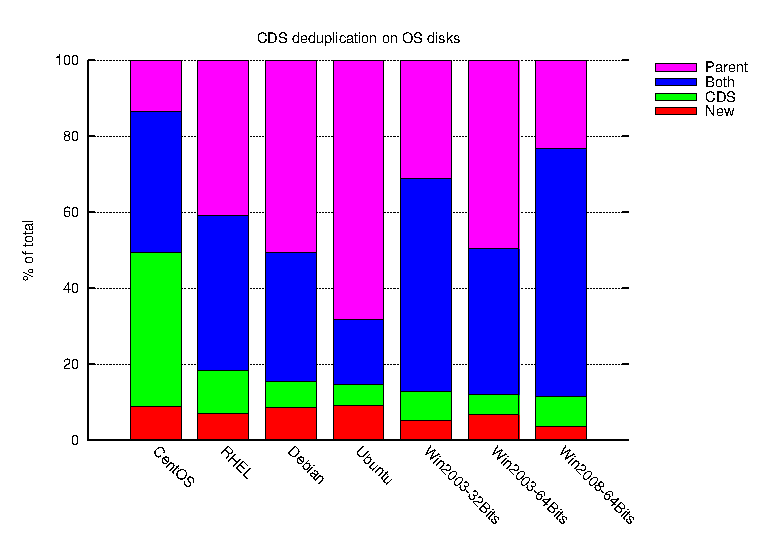
\epsfig{file=images/os_cds_sim.eps, height=2in, width=2.66in}
  \caption{CDS deduplication effect on OS disks}
  \label{fig:oscds}
\end{figure}

For each block, we tag it with one of the following:
\begin{itemize}
\item {New: this block cannot be deduplicated and thus write to block store.}
\item {CDS: this block is deduplicated by CDS.}
\item {Parent: this block is not found in CDS, but is found in parent snapshot's segment recipe.}
\item {Both: this block is both found in CDS and parent snapshot.}
\end{itemize}
As we can see from \ref{fig:oscds}, locality dominates.
This is because the interval between two snapshots is quite short due to our daily snapshot strategy. 
However, locality still doesn't work well on some of the OSes. But CDS, on the contrary,
finds a lot of duplicates that locality can't find, especially in a VM's first snapshot.

Combining all the VMs, we see the overall 7.4TB of data is reduced to 512GB. Extreme bining 
reduces this data set to 542GB, which is slightly worse. As a reference, perfect deduplication achieves
364GB in this experiment.

Overall, none of locality or CDS can solely work well, but by combining them together 
we get fairly good and stable deduplication ratio to all kind of OSes. If compare to all
incremental backup solutions, CDS can save addition 50\%+ of disk space because it greatly reduces
the cross-VM duplicates.

\subsection{Data Disk}
Figure \ref{fig:pd} shows the compression ratio of perfect deduplication at different data scales. 
Basically perfect deduplication would help us save 50\% of space on user data, 
regardless of scale. If we put all these unique data into CDS, we could achieve perfect deduplication, 
which is not affordable. So we need to see how much space saving of perfect 
deduplication can be achieved through a limit size CDS.
\begin{figure}
  \centering
  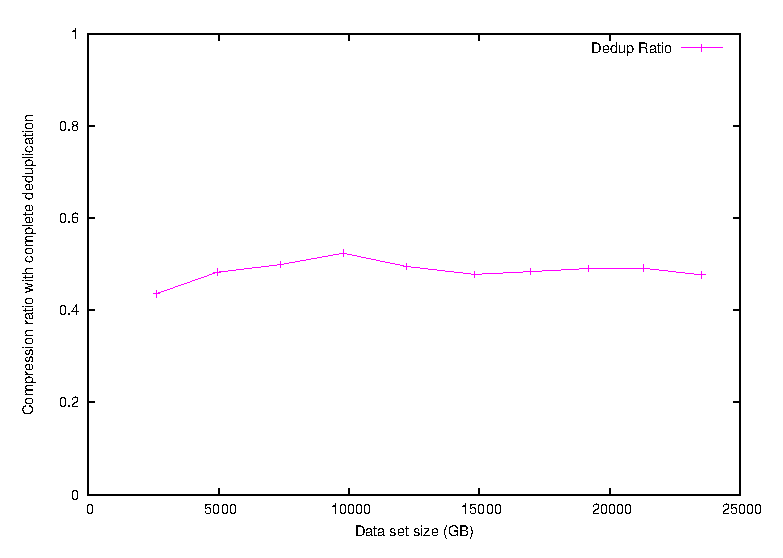
\epsfig{file=images/dedup_ratio.eps, height=2in, width=2.66in}
  \caption{Perfect deduplication on data disks}
  \label{fig:pd}
\end{figure}

We rank unique data blocks by their duplication count, 
and choose the hottest blocks as CDS. 
We define \emph{space saving ratio} as the space saving of CDS divide by 
perfect deduplication saving. Figure \ref{fig:datacdssize} shows the relationship between CDS size and space saving. 
It’s clear a very small amount of CDS data provides more than 50\% saving. 
But this effect decreases when more data are added to CDS. 
The lower bound of CDS space saving ratio is 50\%, which is very easy to accomplish. 

\begin{figure}
  \centering
  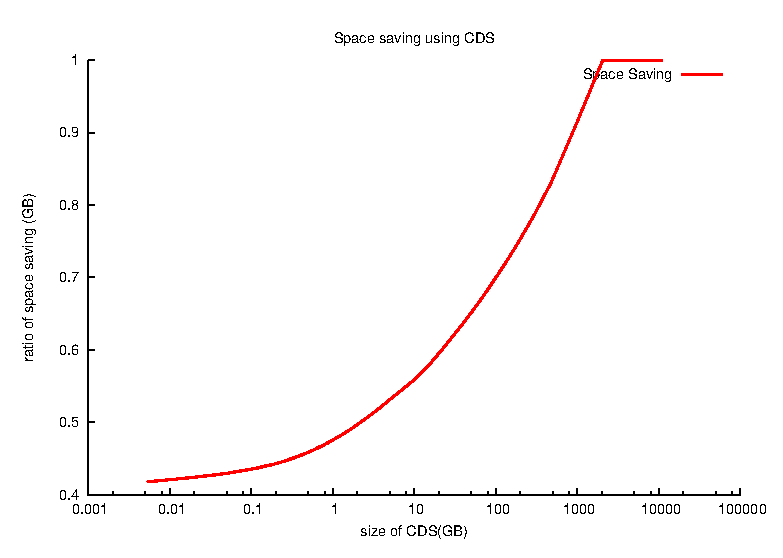
\epsfig{file=images/uniquedata-saving.eps, height=2in, width=2.66in}
  \caption{Size of CDS vesus space saving}
  \label{fig:datacdssize}
\end{figure}

The upper bound of CDS size is restricted by system memory resource.
Figure \ref{fig:datacds} shows how CDS space saving is affected by the system scale. 
In this experiment we first set out a goal of space saving ratio, 
then we watch how much data we need to put into CDS to achieve this goal.
From the graph we can see a 75\% saving goal lead to a stable ratio between 
CDS size and data size, which requires 0.01\% of data to be put in CDS.

Base on above data we can estimate the size of data CDS and its effect. 
Currently we prepared 500MB memory per machine to store CDS meta, then it can represent 50GB of data. 
If we assume each VM has 30GB of user data at runtime, and we host 25 VMs per machine, 
 maintain 10 snapshots per VM, each brings 10\% additional modified data. 
Thus the user data in snapshot system is 1.5TB per machine. So the upper bound of 
$CDS size/ Data size = 0.033$, which is sufficient for the 75\% saving goal.

\begin{figure}
  \centering
  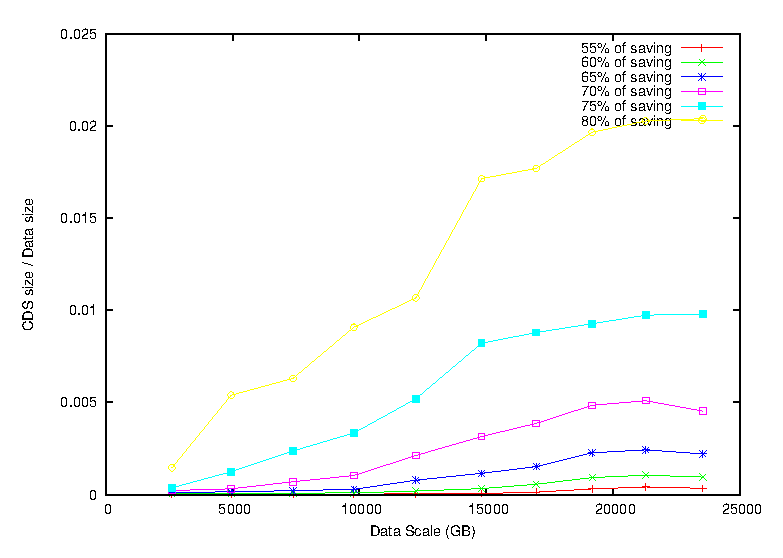
\epsfig{file=images/cds_scale.0.7.eps, height=2in, width=2.66in}
  \caption{CDS deduplication effect on data disks}
  \label{fig:datacds}
\end{figure}

Unlike the CDS of OS disks which is mainly composed of OS related data thus highly predictable, 
data disks is unpredictable because we cannot control what user can put in there. But we still
suspect that highly duplicated data in existing data are very likely to be duplicated again.
So we randomly pick 50 out of 1322 data disks as the new data, and use the rest as existing data
to extract CDS. Using 1.5\% as CDS threshold, we see the total 1198GB of new data is reduced by 
755.8GB, while perfect deduplication can reduce 1017.4GB. So 74.3\% of duplicate blocks are eliminated 
by pre-trained CDS, which is quite satisfiable.

\section{Related Works}
Several approaches have been previously proposed to enable efficient deduplication in D2D backup.

DDFS\cite{bottleneck08} exploits chunk locality to achieve high-throughput perfect deduplication. 
It preserves locality by a Stream-Informed Segment Layout and exploits locality with Locality Preserved Cache. 
An in-memory Bloom Filter is also used to accelerate non-duplicate chunk identification.

Sparse Indexing\cite{sparseindex09} is an approximate deduplication technique designed for D2D backup. 
It divides data stream into variable-sized multiple kilobytes chunks, and construct multiple megabytes segments
using the same chunking technique, 
which are then sampled and mapped to a compact in-memory sparse index. 
Incoming segments are only deduplicated against several existing similar 
segments selected according to the sparse index.

Both DDFS and Sparse Indexing are designed for D2D backup workloads, 
and do not address the scalability issue in a distributed environment. 
A few scalable deduplication approaches have been proposed recently.

Extreme Binning\cite{extreme_binning09} is a scalable parallel deduplication approach 
that targets at non-traditional backup workloads that consist of low-locality individual files. 
It groups highly similar files into bins, and eliminates duplicate chunks inside each bin. 
Duplicate chunks are allowed to exist among different bins, resulting in approximate deduplication. 
By keeping only the primary index in memory, Extreme Binning can reduce the RAM requirement while 
maintaining a reasonably high throughput. However, their per-file based similarity detection 
is going to group all similar files into one node, which will break load balancing if some files are
huge and similar(e.g., virtual machine images).

MAD2\cite{mad210} is a scalable high-throughput exact duplication approach. 
MAD2 utilizes on-disk Hash Bucket Matrix to preserve fingerprint locality and 
integrates in-memory Dual Cache to capture and exploit locality. 
In addition, MAD2 employs Bloom Filter Array to efficiently identify unique 
incoming fingerprints and indicate where a duplicate may reside. 
By employing a DHT-based Load-Balance technique to distribute file recipes 
and chunk contents among multiple storage nodes in their backup sequences, 
MAD2 further enhances performance with a well balanced load. However, the
data locality does not exist for cloud storage because only changed chunks are expected
to be uploaded, and
the heavy usage of memory and CPU indicates such exact deduplication backup systems
need storage-exclusive servers with hardware replication support, which is not a general case 
for the cloud..

HYDRAstor\cite{hydrastor09}, a scalable secondary storage solution, 
constructs its backend using a grid of storage nodes built around a distributed hash table. 
The backend maintains large-scale variable-sized, content-addressed, immutable, 
and highly-resilient data blocks that are logically organized in a directed acyclic graph. 
Duplicate chunks are eliminated according to their hashes. 
HYDRAstor adopts an average chunk size of 64KB, among other constraints, 
to keep all the metadata in memory and avoid the duplicate-lookup disk bottleneck. 
This degrades the space efficiency of deduplication, and still requires huge amount of memory.

We believe a deduplication backend of cloud storage must have scalability and
 high availability built in mind, being able to run on low-cost non-proprietary machines.
  Unlike sloud, all above systems lack one or a few such properties. All exact deduplication approaches
are too costly, this is why we choose similarity based approach to trade deduplication
accuracy for speed. 

Eariler deduplication systems mainly focus on improving storage space efficiency by eliminating 
duplicates at the file level, fixed-size block level, or variable-sized chunk level. 
EMC's Centera\cite{emc_centera} identify and eliminate duplicate data by comparing 
the hash of the whole file or fixed content. Venti\cite{venti02}, a block-level archival storage, 
removes redundant fixed-size data blocks by comparing their secure hashes. Pastiche\cite{pastiche02} 
utilizes chunk-level duplicate detection to construct a resource-saving peer-to-peer backup network. 
Deep Store\cite{deepstore05}, a large scale archival storage system, uses both variable-sized 
chunk-level deduplication and delta compression to save storage. Jumbo Store\cite{jumbo07} organizes 
variable-sized chunks into Hash-Based Directed Acyclic Graphs to save both storage and 
bandwidth while performing incremental upload and versioning for a utility rendering service. 

Duplicate detection technique has also been used in bandwidth-saving synchronization protocols\cite{rsync} 
and low-bandwidth network file systems\cite{lbfs01}.
%\section{Conclusion}
In this paper we present a new parallel deduplication technique for VM cloud.
Our technique utilizes the special data characteristic in VM cloud backup system
to accommodate very limited resources for data deduplication.
By storing the commonly used OS related data, and the hottest user generated data, 
we greatly reduce the cross-VM data duplication in VM snapshot backups. Experiments show
our solution can eliminate the majority of data duplication with a tiny fraction of
block hash index store in memory. It does not only saves valuable system resouces in
the VM cloud, but also makes deduplication much faster.

\bibliographystyle{abbrv}
\bibliography{dedup}
\end{document}
